\documentclass[12pt, letterpaper, twoside]{article}
\usepackage{nopageno,epsfig, amsmath, amssymb}
\usepackage{physics}
\usepackage{mathtools}
\usepackage{hyperref}
\usepackage{xcolor}
\usepackage{mhchem}
\usepackage[normalem]{ulem}
\hypersetup{
    colorlinks,
    linkcolor={blue},
    citecolor={blue},
    urlcolor={blue}
}
\usepackage{empheq}
\usepackage{wrapfig}
\usepackage[shortlabels]{enumitem}

\usepackage[letterpaper,
            margin=0.8in]{geometry}

\newcommand{\psetnum}{2}
\newcommand{\class}{ASTR 531 - Stellar Interiors and Evolution}

\newcommand{\tomtitle}{
    \noindent {\LARGE \fontfamily{cmr}\selectfont \textbf{\class}} \hfill \\[1\baselineskip]
    \noindent {\large \fontfamily{cmr}\selectfont Exam \psetnum \hfill \textsc{Tom Wagg}}\\[0.5\baselineskip]
    {\fontfamily{cmr}\selectfont \textit{\today}}\\[2\baselineskip]
}

\title{\class : Exam \psetnum}
\author{\textbf{Tom Wagg}}

\newcommand{\question}[1]{{\noindent \it #1}}
\newcommand{\answer}[1]{
    \par\noindent\rule{\textwidth}{0.4pt}#1\vspace{0.5cm}
}
\newcommand{\todo}[1]{{\color{red}\begin{center}TODO: #1\end{center}}}

% custom function for adding units
\makeatletter
\newcommand{\unit}[1]{%
    \,\mathrm{#1}\checknextarg}
\newcommand{\checknextarg}{\@ifnextchar\bgroup{\gobblenextarg}{}}
\newcommand{\gobblenextarg}[1]{\,\mathrm{#1}\@ifnextchar\bgroup{\gobblenextarg}{}}
\makeatother

\newcommand{\avg}[1]{\left\langle #1 \right\rangle}
\newcommand{\angstrom}{\mbox{\normalfont\AA}}
\allowdisplaybreaks

\begin{document}

\tomtitle

\vspace{-0.5cm}

\noindent \textbf{[Exam format]}

\noindent This exam is open note but closed book/internet. \textit{[My purpose with this is that students will have written down Eq.\ 28.15 somewhere so can use that but they don't have the full explanations from the book about mass transfer and so will need to explain that themselves]}

\section*{Binary Limbo: How low can you(r separation) go?!}

\question{For each type of mass transfer listed below state whether there is a minimum separation that a binary can achieve during mass transfer.\\
If you answer yes
\begin{itemize}
    \item Explain what physically occurs in the system when it reaches this minimum separation
    \item Find an expression for the minimum separation in terms of the initial separation and initial mass ratio $q = M_{2, i} / M_{1, i}$ (assuming that the rate of mass transfer is constant)
\end{itemize}
If you answer no
\begin{itemize}
    \item Explain why a minimum separation does not exist
\end{itemize}
}

\question{\textbf{Part a - Conservative and Stable Mass Transfer}}
\answer{
    \textbf{Yes}, a minimum separation exists. This minimum occurs when the mass ratio of the binary flips, meaning that the initially more massive star becomes less massive than the secondary star due to the transfer of mass. At this point, the binary stops shrinking and the separation increases instead until mass transfer ends.

    We can find an expression for this point using Eq.\ 28.15 from the textbook. This gives that the change in separation during mass transfer is
    \begin{equation}
        \frac{\dot{a}}{a} = 2 \frac{\dot{M}_1}{M_1} \qty(\frac{M_1}{M_2} - 1)
    \end{equation}
    Therefore, since we are assuming that the mass transfer rate is constant, we can integrate this to find the minimum separation.
    \begin{align}
        \int_{a_i}^{a_{\rm min}} \frac{1}{a} \dd{a} &= 2 \frac{\dot{M}_1}{M_1} \qty(\frac{M_1}{M_2} - 1) \int_0^{t_{\rm min}} \dd{t} \\
        \ln \frac{a_{\rm min}}{a_i} &= 2 \frac{\dot{M}_1}{M_1} \qty(\frac{M_1}{M_2} - 1) \cdot t_{\rm min}
    \end{align}
    The time at which the minimum occurs is the time at which the masses are equal. Therefore, this time is when half the difference in their initial masses has been transferred and so
    \begin{equation}
        t_{\rm min} = -\frac{M_1 - M_2}{2 \dot{M}_1}
    \end{equation}
    where the negative sign accounts for the fact that $\dot{M}_1$ is negative. Putting this all together and substituting $q$ we find that
    \begin{align}
        \ln \frac{a_{\rm min}}{a_i} &= 2 - q - \frac{1}{q} \\
        \Aboxed{ a_{\rm min} &= a_i \, e^{2 - q - \frac{1}{q}} }
    \end{align}
    This function is plotted in Figure~\ref{fig:min_sep} for students reading the solutions who are interested but this is of course not necessary in their answer.
    \begin{figure}
        \centering
        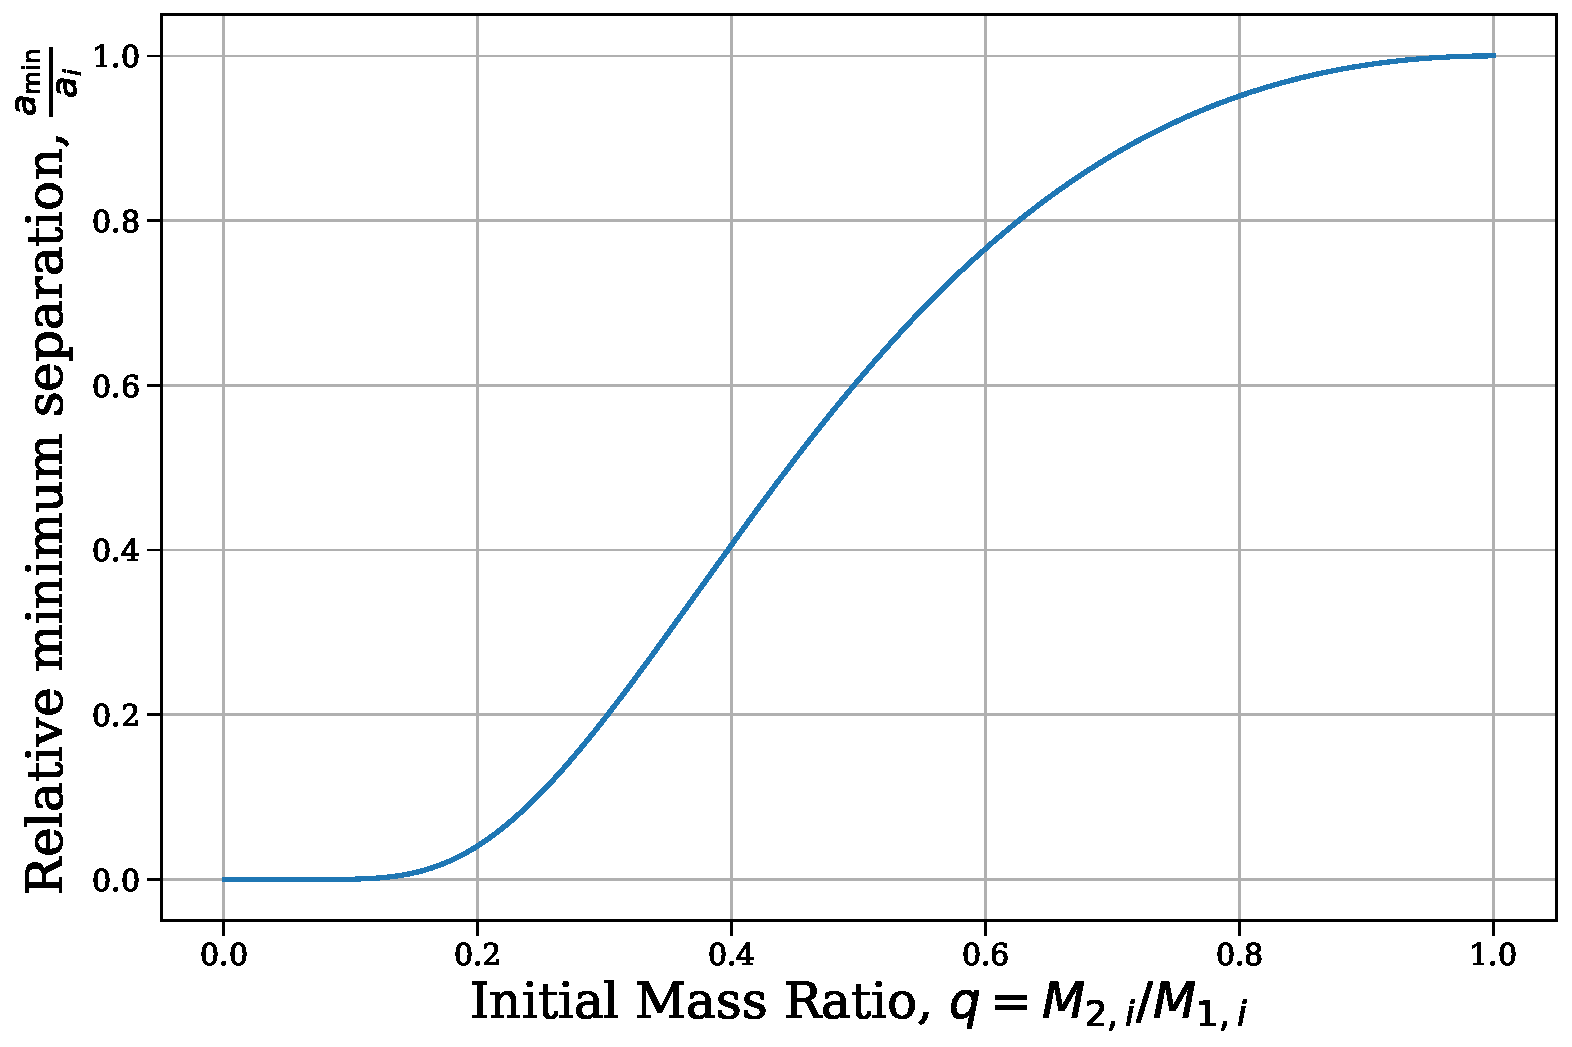
\includegraphics[width=0.8\textwidth]{relative_min_separation.pdf}
        \caption{Minimum separation relative to initial separation for different initial mass ratios (for conservative, stable mass transfer at a constant rate).}
        \label{fig:min_sep}
    \end{figure}
}

\question{\textbf{Part b - Dynamically Unstable Mass Transfer}}
\answer{
    \textbf{No}, there is no minimum separation for dynamically unstable mass transfer. This is because this is a runaway mass transfer process. The donor star does not contract sufficiently (or even expands further) and so does not balance with its shrinking Roche Lobe and thus the mass transfer becomes so fast that the donor star is no longer in hydrostatic equilibrium.

    This leads to an extremely high mass transfer rate such that soon \textit{both} stars overflow their Roche Lobes and this initiates a common envelope event. This common envelope is the reason that no minimum separation exists. The stars orbit through the gas of the common envelope which results in friction and dramatically decreases the orbital separation. There is no limit to how close this effect may drive the stars, indeed in many cases a common envelope leads to a stellar merger in which the stars merge entirely and thus have zero orbital separation.
}

\end{document}

 